\begin{figure*}[t] 
\centering
\begin{tikzpicture}[
   scale=0.7,
    node distance=6mm,
    io/.style={circle, draw, minimum size=4.5mm, inner sep=0pt},
    hid/.style={rounded corners, draw, fill=black!4,
                minimum width=10mm, minimum height=34mm, align=center},
    norm/.style={rounded corners, draw, fill=black!8,
                 minimum width=6mm, minimum height=34mm, align=center},
    >=stealth
]

% --- vhodni sloj (12 nevronov) ---
\foreach \i in {1,...,6}
    \node[io] (in\i) at (0, {2.5 - \i*0.7}) {};
\node[left=2mm of in1] (lbl1) {\footnotesize nagib};
\node[left=2mm of in2] (lbl2) {\footnotesize kotna hitrost nagiba};
\node[left=2mm of in3] (lbl3) {\footnotesize naklon};
\node[left=2mm of in4] (lbl4) {\footnotesize kotna hitrost naklona};
\node[left=2mm of in5] (lbl5) {\footnotesize odmik po x osi};
\node[left=2mm of in6] (lbl6) {\footnotesize linearna hitrost};              

% --- normalizacija (fiksne konstante) ---
\node[norm] (nrm) at (1.5, 0.0) {\rotatebox{90}{\footnotesize normalizacija}};

% --- skrita sloja (bloka) ---
\node[hid] (h1) at (3.5, 0.00) {GRU \\ + \\MLP};

% --- izhodni sloj (3 nevroni) ---
\node[io] (out1) at (6, 1.8) {};
\node[io] (out2) at (6, 0.9) {};
\node[io] (out3) at (6, 0) {};
\node[io] (out4) at (6, -0.9) {};
\node[io] (out5) at (6, -1.8) {};
\node[right=2mm of out1] (lblo1) {\footnotesize kot motorja M1};
\node[right=2mm of out2] (lblo2) {\footnotesize kot motorja M2};
\node[right=2mm of out3] (lblo3) {\footnotesize tok motorja M3};
\node[right=2mm of out4] (lblo4) {\footnotesize kot motorja M4};
\node[right=2mm of out5] (lblo5) {\footnotesize kot motorja M5};

% --- normalizacija (fiksne konstante) ---
\node[norm] (nrm2) at (10.5, 0.00) {\rotatebox{90}{\footnotesize normalizacija}};

% --- slika simulacije
\node[inner sep=0pt] (simulation) at (13.8, 0) {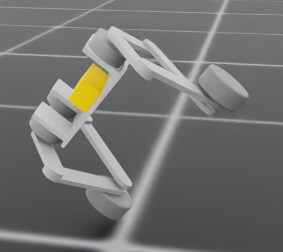
\includegraphics[width=.18\textwidth]{Images/Simulation.png}}; 
\node[above=1mm of simulation] {Simulacija};

% --- povezave ---
\foreach \i in {1,...,6}
    \draw[->, black!70] (in\i.east) -- (nrm.west |- in\i.east);
\draw[->, black!60] (nrm.east) -- (h1.west);
\foreach \o in {1,2,3,4,5}
    \draw[->, black!70] (h1.east) -- (out\o.west);;
\foreach \o in {1,2,3,4,5}
    \draw[->, black!70] (lblo\o.east) -- (nrm2.west |- out\o.east);

\draw[->, black!70] (nrm2.east) -- (simulation.west);
\draw[black!70] (simulation.south) |- (-4.5, -2.5) -- (-4.5, 1.8);

\foreach \i in {1,...,6}
    \draw[->, black!70] (-4.5, {2.5 - \i*0.7}) -- (lbl\i.west);

\draw[->, dashed, black, thick] (simulation.north west) -- ++(0,0.8) -| (h1.north) 
    node[pos=0.2, above] {Nagrada $R_{1,2}$};

\end{tikzpicture}
\caption{Arhitektura strategije: 6-razsežni vektor stanja se najprej normira
s fiksnimi konstantami, sledi obdelava z RNN nevronsko mrežo, normalizacija izhodnih veličin in simulacija. 
3 izhodne krmilne veličine.}
\label{nevronska mreža}
\end{figure*} 